\chapter{Use Cases \\
\small{\textit{Chan, Moks, Ponte}}
\index{use cases} 
\index{Chapter!Use Cases}
\label{Chapter::UseCases}}

This chapter presents the use case diagrams that satisfy the system requirements. Each use case is mapped to at least one requirement, with preconditions, flows, and postconditions defined. All use cases assume the system is run locally, either through a command-line interface, Python environment, or an optional locally hosted interface on \texttt{localhost}.


\section{Table of Use Cases}
\small
\begin{longtable}{|p{1.5cm}|p{3cm}|p{8.5cm}|p{1.5cm}|}
\caption{Use Cases Table \label{Table::UseCases}}\\
\hline
\textbf{Use Case} & \textbf{Requirements} & \textbf{Name and Description} & \textbf{Activity Diagrams}\\
\hline
\endhead

\UseCaseReference{ucTranslatePrompt} &
\RequirementReference{reqkFunctional}{reqfTranslation},
\RequirementReference{reqkQuality}{reqqSchemaValid} &
\UseCaseName{ucTranslatePrompt}:~Convert a natural language optimization prompt into schema-valid JSON and compile it into a QUBO model ready for a solver. &
\ref{fig:UC-1 Translate} \\
\hline

\UseCaseReference{ucReverseTranslate} &
\RequirementReference{reqkFunctional}{reqfReverseTranslate},
\RequirementReference{reqkQuality}{reqqFidelity} &
\UseCaseName{ucReverseTranslate}:~Reconstruct natural language from the QUBO/JSON and compute a fidelity score to show how well it matches the user’s intent. &
\ref{fig:UC-2 Reverse Translate} \\
\hline

\UseCaseReference{ucExecuteReport} &
\RequirementReference{reqkFunctional}{reqfExecution},
\RequirementReference{reqkFunctional}{reqfReporting} &
\UseCaseName{ucExecuteReport}:~Run the QUBO on a simulator or solver and return the best solution, constraint satisfaction, and runtime, saving outputs for reuse. &
\ref{fig:UC-3 Execute Report} \\
\hline

\UseCaseReference{ucViewLogsMetrics} &
\RequirementReference{reqkFunctional}{reqfReporting},
\RequirementReference{reqkQuality}{reqqLatency},
\RequirementReference{reqkQuality}{reqqSchemaValid} &
\UseCaseName{ucViewLogsMetrics}:~Display and download logs, success rates, latency, and fidelity plots to support reproducibility and analysis. &
\ref{fig:UC-4 View Logs Metrics} \\
\hline

\UseCaseReference{ucManagePromptLibrary} &
\RequirementReference{reqkFunctional}{reqfPromptLibrary} &
\UseCaseName{ucManagePromptLibrary}:~Allow the team to add, update, and tag benchmark prompts by problem type for consistent testing. &
\ref{fig:UC-5 Manage Prompt Library} \\
\hline

\end{longtable}



\section{Detailed Use Case Examples}

% =====================================
% UC-1
% =====================================
\begin{table}[H]
\center
\caption{\TableLabel{ucTranslatePrompt}. \UseCaseNameWIReference{ucTranslatePrompt}{UC-1} Translate NL to QUBO}
\scalebox{1}{
\begin{tabular}{|p{16cm}|}
\hline
\begin{useCase}[\UseCaseNameWIReference{ucTranslatePrompt}{UC-1} Translate NL to QUBO]
\UseCaseLabel{ucTranslatePrompt}{UC-1}
\index{UseCase!UC-1 Translate NL to QUBO}
Turns a natural language optimization prompt into schema-valid JSON and compiles it into a QUBO model.
\end{useCase} \\
\hline
Requirements: \RequirementReference{reqkFunctional}{reqfTranslation}, \RequirementReference{reqkQuality}{reqqSchemaValid} \\
\hline
Brief description: \\
User provides a plain-English prompt (e.g., "Assign 20 technicians to 4 shifts") and the system generates schema-valid QUBO JSON plus a compiled QUBO. \\
\hline
Primary actors: User \\
\hline
Secondary actors: LLMClient, QUBOTranslator, QUBOCompiler \\
\hline
Preconditions: User has launched the local system interface (CLI, Python script, or locally hosted UI); LLM service available. \\
\hline
Main flow:
\begin{enumerate}
\item User submits natural language prompt.
\item System translates to JSON.
\item JSON validated against schema.
\item Compiled into QUBO model.
\end{enumerate} \\
\hline
Postconditions: Valid QUBO model ready for solving. \\
\hline
Alternative flows: Invalid JSON → error message; compilation fails → fallback. \\
\hline
\end{tabular}}
\end{table}

% =====================================
% UC-2
% =====================================
\begin{table}[H]
\center
\caption{\TableLabel{ucReverseTranslate}. \UseCaseNameWIReference{ucReverseTranslate}{UC-2} Reverse Translate \& Score}
\scalebox{1}{
\begin{tabular}{|p{16cm}|}
\hline
\begin{useCase}[\UseCaseNameWIReference{ucReverseTranslate}{UC-2} Reverse Translate \& Score]
\UseCaseLabel{ucReverseTranslate}{UC-2}
\index{UseCase!UC-2 Reverse Translate \& Score}
Reconstruct a QUBO into natural language and compute a fidelity score.
\end{useCase} \\
\hline
Requirements: \RequirementReference{reqkFunctional}{reqfReverseTranslate}, \RequirementReference{reqkQuality}{reqqFidelity} \\
\hline
Primary actors: User \\
\hline
Secondary actors: LLMClient, QUBOReverseTranslator, FidelityCalculator \\
\hline
Preconditions: Valid QUBO JSON available. \\
\hline
Main flow:
\begin{enumerate}
\item System takes compiled QUBO JSON.
\item Reverse translator reconstructs natural language description.
\item FidelityCalculator computes similarity against the original prompt.
\end{enumerate} \\
\hline
Postconditions: Fidelity score available to the user. \\
\hline
Alternative flows: Low fidelity score → flagged result with warning. \\
\hline
\end{tabular}}
\end{table}

% =====================================
% UC-3
% =====================================
\begin{table}[H]
\center
\caption{\TableLabel{ucExecuteReport}. \UseCaseNameWIReference{ucExecuteReport}{UC-3} Execute \& Report}
\scalebox{1}{
\begin{tabular}{|p{16cm}|}
\hline
\begin{useCase}[\UseCaseNameWIReference{ucExecuteReport}{UC-3} Execute \& Report]
\UseCaseLabel{ucExecuteReport}{UC-3}
\index{UseCase!UC-3 Execute \& Report}
Run QUBO on simulator/solver and return solutions with reports.
\end{useCase} \\
\hline
Requirements: \RequirementReference{reqkFunctional}{reqfExecution}, \RequirementReference{reqkFunctional}{reqfReporting} \\
\hline
Primary actors: User \\
\hline
Secondary actors: LocalSolver, DWaveSolver, ResultWriter \\
\hline
Preconditions: Compiled QUBO available. \\
\hline
Main flow:
\begin{enumerate}
\item User requests execution of compiled QUBO.
\item System runs QUBO on simulator by default.
\item (Optional) If hardware solver is available, extend to D-Wave execution.
\item Collect objective value, assignment, feasibility, and runtime.
\item Save results and metrics for later retrieval.
\end{enumerate} \\
\hline
Postconditions: Results stored and available for analysis. \\
\hline
Alternative flows: Solver unavailable → error returned; execution timeout → fallback. \\
\hline
\end{tabular}}
\end{table}

% =====================================
% UC-4
% =====================================
\begin{table}[H]
\center
\caption{\TableLabel{ucViewLogsMetrics}. \UseCaseNameWIReference{ucViewLogsMetrics}{UC-4} View Logs \& Metrics}
\scalebox{1}{
\begin{tabular}{|p{16cm}|}
\hline
\begin{useCase}[\UseCaseNameWIReference{ucViewLogsMetrics}{UC-4} View Logs \& Metrics]
\UseCaseLabel{ucViewLogsMetrics}{UC-4}
\index{UseCase!UC-4 View Logs \& Metrics}
View or download logs, success rates, latency, and fidelity plots.
\end{useCase} \\
\hline
Requirements: \RequirementReference{reqkFunctional}{reqfReporting}, \RequirementReference{reqkQuality}{reqqLatency}, \RequirementReference{reqkQuality}{reqqSchemaValid} \\
\hline
Primary actors: User \\
\hline
Secondary actors: ResultMetrics, Visualization \\
\hline
Preconditions: Logs and metrics exist from previous executions. \\
\hline
Main flow:
\begin{enumerate}
\item User requests logs and metrics.
\item System fetches stored data.
\item System displays results through the local interface (CLI output, local visualization window, or locally hosted dashboard) and/or allows export as CSV/plots.
\end{enumerate} \\
\hline
Postconditions: Logs and visualizations delivered to user. \\
\hline
Alternative flows: Logs unavailable → system returns “no data available.” \\
\hline
\end{tabular}}
\end{table}

% =====================================
% UC-5
% =====================================
\begin{table}[H]
\center
\caption{\TableLabel{ucManagePromptLibrary}. \UseCaseNameWIReference{ucManagePromptLibrary}{UC-5} Manage Prompt Library}
\scalebox{1}{
\begin{tabular}{|p{16cm}|}
\hline
\begin{useCase}[\UseCaseNameWIReference{ucManagePromptLibrary}{UC-5} Manage Prompt Library]
\UseCaseLabel{ucManagePromptLibrary}{UC-5}
\index{UseCase!UC-5 Manage Prompt Library}
Add, update, and tag benchmark prompts by problem type.
\end{useCase} \\
\hline
Requirements: \RequirementReference{reqkFunctional}{reqfPromptLibrary} \\
\hline
Primary actors: User \\
\hline
Secondary actors: PromptDataset \\
\hline
Preconditions: Prompt library available. \\
\hline
Main flow:
\begin{enumerate}
\item User adds a new prompt or selects an existing one.
\item User edits or tags the prompt with problem type.
\item System saves changes and updates library.
\end{enumerate} \\
\hline
Postconditions: Prompt library updated successfully. \\
\hline
Alternative flows: Invalid prompt → rejected with error; duplicate prompt → flagged for review. \\
\hline
\end{tabular}}
\end{table}

% =====================================
% UC Figure
% =====================================
\begin{figure}[H]
    \centering
    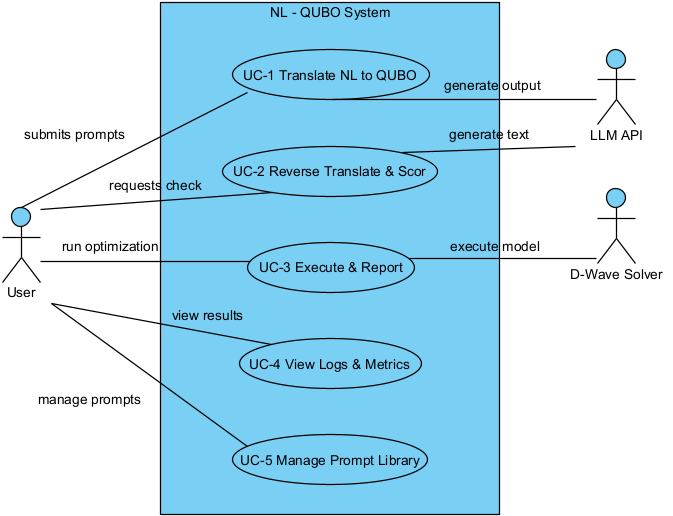
\includegraphics[width=0.8\textwidth]{png/ucdiagram.png} % <-- replace with your file name
    \caption{Use Case Diagram for the NL--QUBO System showing the five core user interactions.}
    \label{fig:uc1-diagram}
\end{figure}


\section{Activity Diagrams}

\begin{figure}[H]
    \centering
    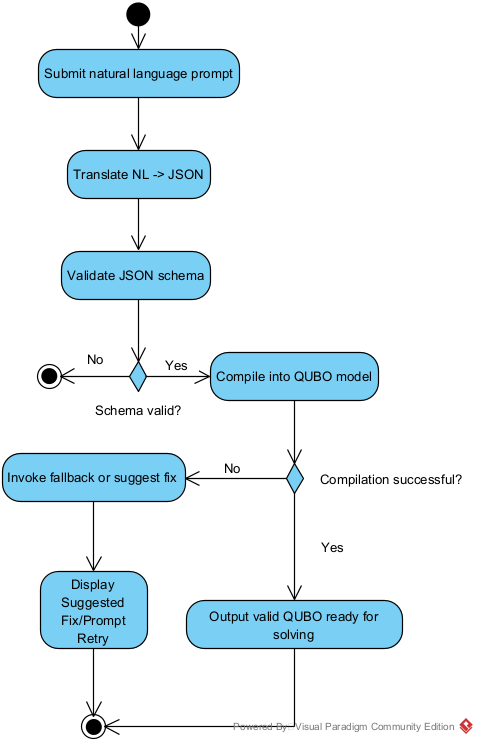
\includegraphics[width=.5\linewidth]{png/UC-1 Translate NL to QUBO.png}
    \caption{Activity Diagram for \UseCaseNameWIReference{ucTranslatePrompt}}
    \label{fig:UC-1 Translate}
\end{figure}

\subsection{Activity Diagram 1 Description}
In this activity, the workflow begins when the user interfaces with the system through the main controller or UI, which passes the written natural-language prompt into the system as a Prompt object. The LLMClient sends this prompt to the language model, while the QUBOTranslator structures the request, parses the response, and converts the returned text into a JSON-formatted representation of variables, constraints, and the optimization objective. Once JSON is obtained, a validation step is performed by SchemaValidator to ensure that the output conforms to the expected QUBO schema. After validation succeeds, the QUBOCompiler converts the JSON into an internal QUBOModel (or BQM) that stores coefficients and variable names, making it executable by downstream solver classes.

\begin{figure}[H]
    \centering
    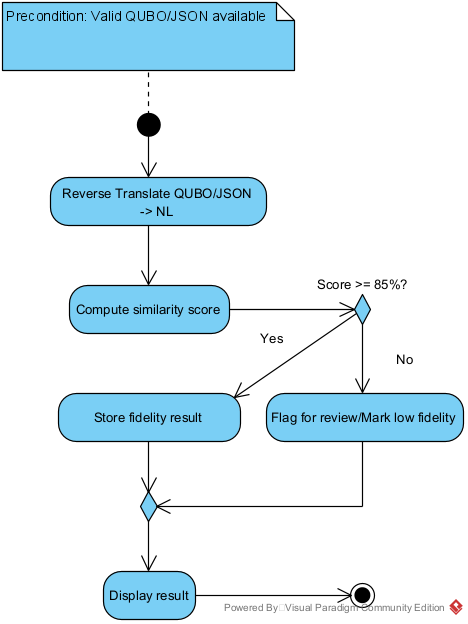
\includegraphics[width=.5\linewidth]{png/UC-2 Reverse Translate & Score.png}
    \caption{Activity Diagram for \UseCaseNameWIReference{ucReverseTranslate}}
    \label{fig:UC-2 Reverse Translate}
\end{figure}

\subsection{Activity Diagram 2 Description}
This activity begins with the previously compiled QUBOModel, selected by the UI or controller. The QUBOReverseTranslator inspects the model’s internal structure and constructs an LLM prompt that describes the model’s objective and constraints, relying again on the LLMClient to convert the structured representation back into natural language. The output description is then passed to the FidelityCalculator, which compares it against the original Prompt and computes a similarity score based on embeddings, token overlap, or other comparison metrics. The resulting fidelity score, along with the reconstructed description, is stored in Result and ResultMetrics objects so the system can track model interpretability and correctness across runs.

\begin{figure}[H]
    \centering
    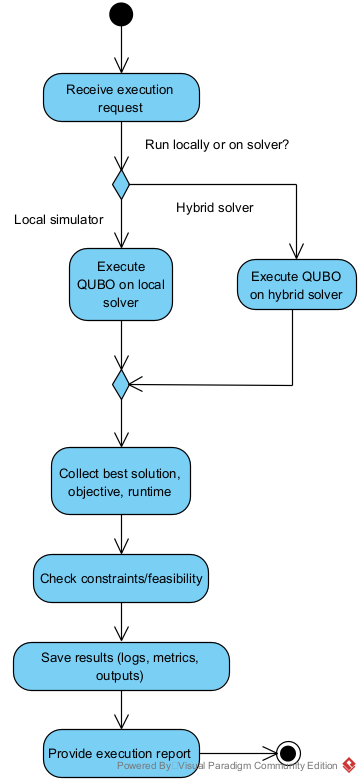
\includegraphics[width=.5\linewidth]{png/UC-3 Execute & Report.png}
    \caption{Activity Diagram for \UseCaseNameWIReference{ucExecuteReport}}
    \label{fig:UC-3 Execute Report}
\end{figure}

\subsection{Activity Diagram 3 Description}
When the user chooses to execute a compiled model, the UI/controller retrieves the corresponding QUBOModel and dispatches it to the chosen solver. The default solver is the LocalSolver, which performs classical simulation on the model, whereas DWaveSolver may be invoked for hardware execution if configured. These solver classes evaluate the model using the stored coefficients and return solutions including binary assignments, objective values, constraint violations, timing information, and hardware metadata. The controller then passes solver output to Result and ResultMetrics, which store structured data about performance and correctness. Finally, ResultWriter persists these results to files or logs so they can be aggregated, visualized, and compared across experiments.

\begin{figure}[H]
    \centering
    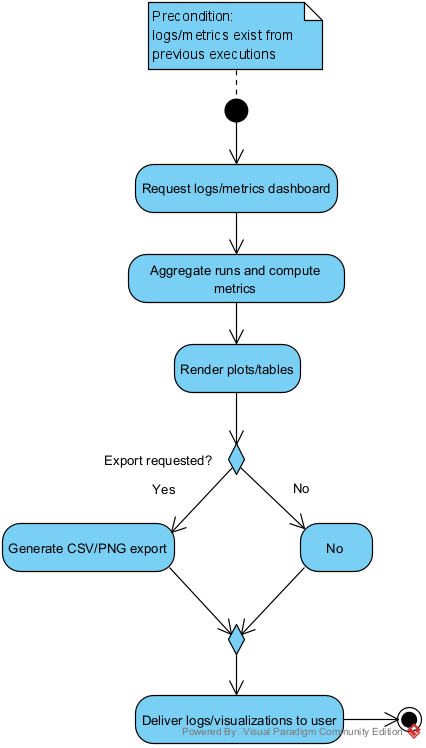
\includegraphics[width=.5\linewidth]{png/UC-4 View Logs & Metrics.png}
    \caption{Activity Diagram for \UseCaseNameWIReference{ucViewLogsMetrics}}
    \label{fig:UC-4 View Logs Metrics}
\end{figure}

\subsection{Activity Diagram 4 Description}
Here, the user interacts through the UI/controller to request previous results or analytics. The controller queries ResultMetrics to retrieve aggregated statistics such as fidelity distributions, runtime comparisons, success rates, and solver-to-solver differences. Raw logs and run histories come from stored Result objects and files written by ResultWriter. When the user requests visual output, the Visualization class generates charts (e.g., histograms, scatter plots, line graphs) or exports tables suitable for CSV/analysis pipelines. The UI then displays these results in textual or graphical form, allowing users to compare runs or export data.

\begin{figure}[H]
    \centering
    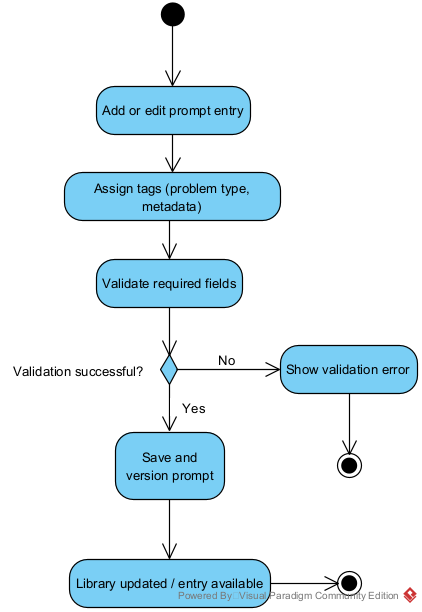
\includegraphics[width=.5\linewidth]{png/UC-5 Manage Prompt Library.png}
    \caption{Activity Diagram for \UseCaseNameWIReference{ucManagePromptLibrary}}
    \label{fig:UC-5 Manage Prompt Library}
\end{figure}

\subsection{Activity Diagram 5 Description}

This activity allows users to create, edit, tag, or select existing prompts for benchmarking. The UI/controller enables selection from the PromptLibrary, which store all prompt templates along with metadata like problem type, tags, and optional ground-truth information. When editing occurs, the Prompt object is updated with new structure or content, and changes are stored back into the dataset. If prompts are linked to experiment runs or fidelity evaluations, ResultWriter may log updates so comparisons between model versions remain traceable. The PromptLibrary ensures that prompts remain organized and retrievable across future workflows like translation, execution, and reverse translation.

